\chapter{Appendix 2 - Instrukcja instalacji systemu}

	\section{Aplikacja serwerowa}
	
	Pierwszym krokiem do uruchomienia systemu jest skonfigurowanie systemu. Aplikacja serwerowa jest dostarczona jako \textit{Web Deployment Package}, który należy wdrożyć (klikając prawym przyciskiem myszy i wybierając "Wdróż") do stworzonej wcześniej witryny w menedżerze internetowych usług informacyjnych (\textit{IIS}). 
	\begin{figure}[H]			
		\centering
		\caption{Okno menedżera internetowych usług informacyjnych. Na czerwono oznaczone zostało miejsce, w którym będzie znajdowała się nasza strona. Na niebiesko oznaczono ikonę włączania usługi.}
		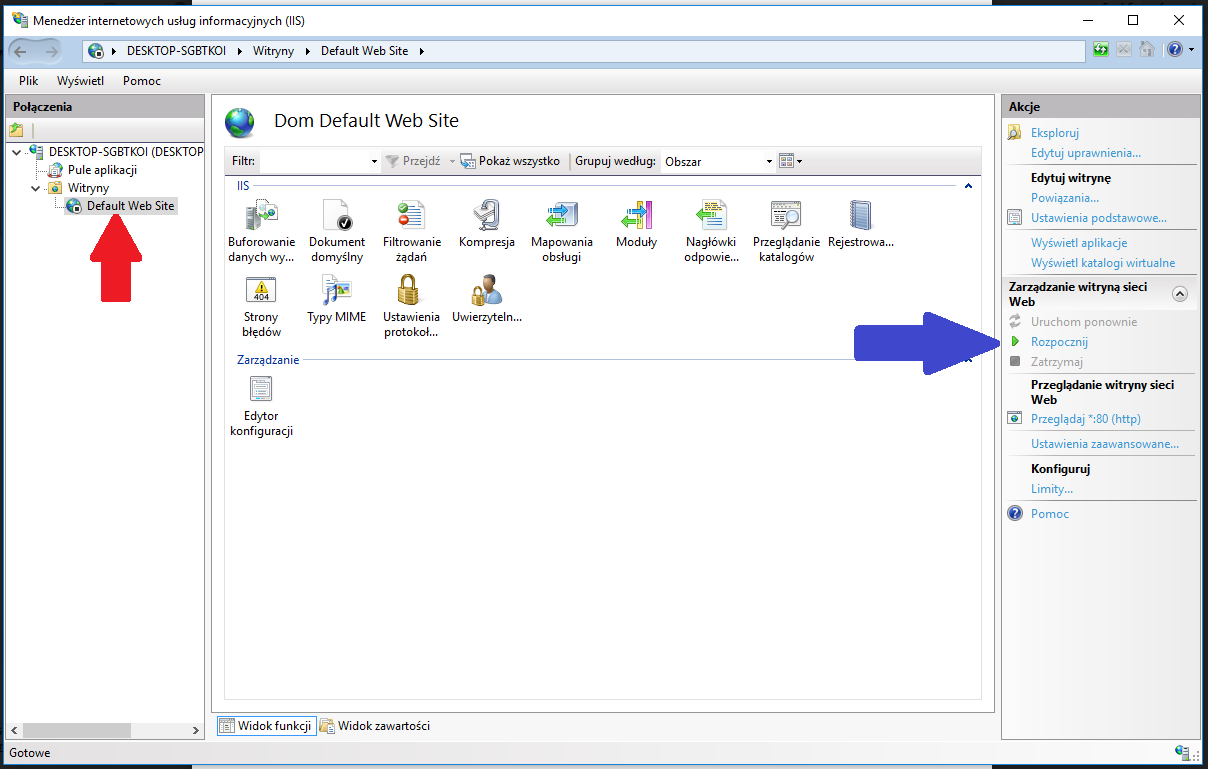
\includegraphics[width=1.0\textwidth]{iis}
	\end{figure}
	Kiedy aplikacja zostanie poprawnie wdrożona, należy skonfigurować dane dostępowe do bazy danych poprzez edycję \textit{'connection-string'} w pliku Web.config w folderze serwera. Po tej operacji należy zrestartować serwer.\\	
	
	\section{Konfiguracja bazy danych}
	
	Aplikacja współpracuje z bazą danych PostgreSQL. Aby utworzyć wymagane przez serwer struktury bazodanowe, należy wywołać w utworzonej dla systemu bazie danych skrypt SQL. Znajduje się on w pliku \textit{'script.sql'} i dostarczony jest on wraz plikiem wdrożeniowym serwera.
		
	
	\section{Aplikacja kliencka}
	
	Aplikacje kliencką należy włączyć z uprawnieniami administratora. Przed uruchomieniem aplikacji administracyjnej, należy skonfigurować dane znajdujące się w pliku \textit{'config.xml'}. W danej \textit{'PictureLocation'} należy podać względną ścieżkę do mapy, odnosząc się do folderu, w którym znajduje się wykonywalna aplikacja. Do danej \textit{'ServerIp'} należy przypisać adres ip serwera wraz z portem, zaś w \textit{ClientIp} należy wstawić adres ip klienta, bez portu. Dane \textit{'Login'} i \textit{'Password'} są opcjonalne i zawierają zapamiętane dane logowania, którymi wypełniane jest pierwsze okno aplikacji. Po włączeniu aplikacji i zalogowaniu się (domyślne dane logowania to \textit{'admin'} i \textit{'admin'}), okno konfiguracji pozwala na bardziej rozbudowaną konfigurację systemu.\\
	Wciśnięcie przycisku 'Konfiguracja' (reprezentowane w oknie jako ikona dwóch trybów), otwiera osobne okno, pozwalające na konfigurację kluczowych elementów systemu.\\
	Pierwszy panel w oknie konfiguracji pozwala na edycję fizycznej wielkości systemu oraz danych na temat transmiterów (umożliwia również ich dodawanie oraz usuwanie).
	\begin{figure}[H]			
		\centering
		\caption{Panel edycji transmiterów}
		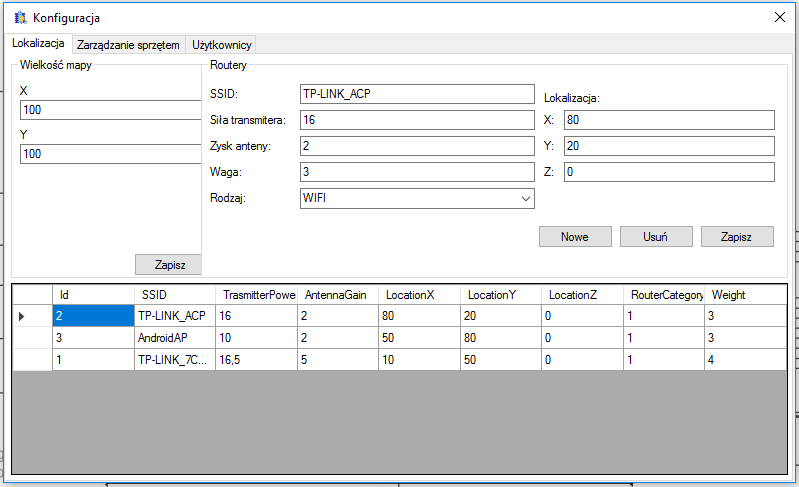
\includegraphics[width=0.75\textwidth]{panel_konf_router}
	\end{figure}
	W dolnej części okna wyświetlone są wszystkie zarejestrowane routery. Wciśnięcie wybranego z nich powoduje przejście do trybu edycji - pola edycji routerów zostaną wypełnione danymi wybranego urządzenia. Należy wprowadzić wymagane dane i nacisnąć przycisk "Zapisz".\\
	Drugi panel pozwala na definiowanie i edycję urządzeń sterowanych.
	\begin{figure}[H]			
		\centering
		\caption{Panel edycji urządzeń}
		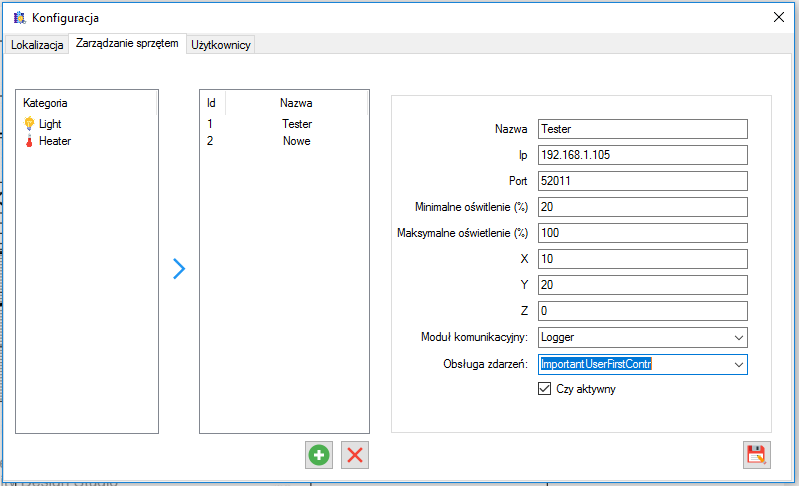
\includegraphics[width=0.75\textwidth]{panel_konf_ster}
	\end{figure}
	Wszystkie urządzenia zarejestrowane w systemie podzielone są na kategorie.	Aby przejść do widoku wyświetlania i edycji danych urządzenia, należy wybrać kategorię urządzenia, a następnie wybrać interesującą nas pozycję ze środkowego panelu. Powoduje to pojawienie się w prawym panelu formularza z danymi danego urządzenia. Formularze są tworzone dynamicznie, a rodzaj i ilość ich pól zależne są od kategorii urządzenia.\\	
	Ostatni panel to panel użytkowników. Są to osoby, które korzystały z aplikacji mobilnej, a ich pozycja została chociaż raz obliczona. Użytkownicy będą tam pojawiać wraz z czasem, a ich konfiguracja nie jest wymagana do poprawnego działania systemu.
	\begin{figure}[H]			
		\centering
		\caption{Panel edycji użytkowników}
		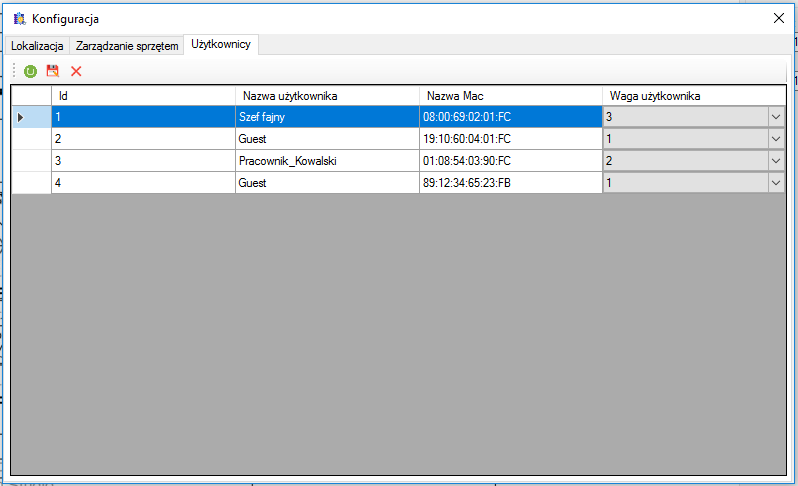
\includegraphics[width=0.75\textwidth]{panel_konf_users}
	\end{figure}
	Widok pozwala na podglądnięcie użytkowników oraz na zmianę ich nazwy oraz wagi. Nazwa pozwala na rozróżnianie użytkowników w sposób łatwiejszy niż adres MAC. Waga odgrywa kluczową rolę podczas obliczania parametrów do sterowania urządzeniami - czym wyższa waga użytkownika, tym większe ma on znaczenie dla urządzenia, w którego zasięgu znajduje się obliczona lokalizacja. Dodatkowo, pojawienie się użytkownika o określonej wadze może mieć wpływ na zajście zdarzenia, zdefiniowanego dla urządzenia.\\
		
	\section{Aplikacja mobilna}
	
	Aplikację instaluje się przy użyciu pliku \textit{.apk}. Aplikacja mobilna, po zainstalowaniu w telefonie, wymaga wpisania adresu ip i portu serwera. Serwis lokalizujący włącza się przy użyciu przycisku w MainActivity.
	\begin{figure}[H]			
		\centering
		\caption{Ekran konfiguracyjny aplikacji mobilnej}
		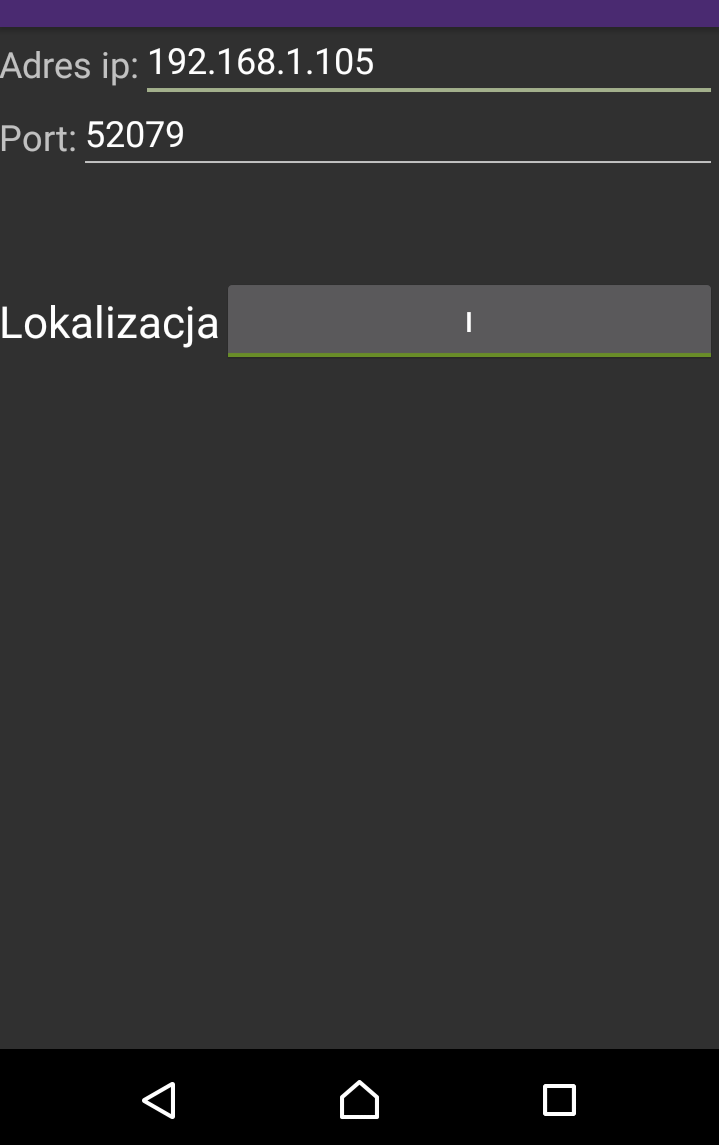
\includegraphics[width=0.3\textwidth]{apk_mobilna}
	\end{figure}